\documentclass[11pt,a4paper]{article}
\usepackage[margin=25mm,headheight=15pt]{geometry}
\usepackage{fontspec}
\setmainfont{texgyretermes}[Extension=.otf,UprightFont=*-regular,BoldFont=*-bold,ItalicFont=*-italic,BoldItalicFont=*-bolditalic]
\usepackage{unicode-math}
\setmathfont{texgyretermes-math.otf}
\usepackage{graphicx,booktabs,tabularx,longtable,array,amsmath,amsthm}
\usepackage{xcolor,enumitem,microtype,fancyhdr,caption,float}
\usepackage{xurl}
\usepackage[hidelinks,unicode]{hyperref}
\definecolor{slate}{HTML}{354B55}
\definecolor{sage}{HTML}{687767}
\definecolor{copper}{HTML}{A46542}
\usepackage{titlesec}
\titleformat{\section}{\Large\bfseries\color{slate}}{\thesection}{0.7em}{}
\titleformat{\subsection}{\large\bfseries}{\thesubsection}{0.7em}{}
\setlength{\parindent}{0pt}
\setlength{\parskip}{6pt plus 1pt minus 1pt}
\setlength{\emergencystretch}{2em}
\linespread{1.10}
\setlist{nosep,leftmargin=1.5em}
\setcounter{tocdepth}{1}
\captionsetup{font=small,labelfont=bf,justification=raggedright,singlelinecheck=false}
\pagestyle{fancy}\fancyhf{}
\fancyhead[L]{\small\color{slate}Checkers with Runway 13}
\fancyhead[R]{\small\color{slate}Working white paper · v1}
\fancyfoot[C]{\small\thepage}
\renewcommand{\headrulewidth}{0.3pt}
\newcommand{\R}{\mathbb R}
\newcommand{\status}[1]{\par\smallskip\noindent\textbf{Evidence status.} #1\par\smallskip}
\newtheorem{proposition}{Proposition}
\hypersetup{pdftitle={Checkers with Runway 13: Reconstructing Kai Tak's Approach},pdfauthor={Aryan Ayyar},pdfsubject={Working white paper, version 1, 13 October 2026}}
\begin{document}
\hypersetup{pageanchor=false}
\begin{titlepage}
\vspace*{18mm}
{\large\color{sage}RESEARCH WHITE PAPER · FIRST WORKING DRAFT\par}
\vspace{12mm}
{\fontsize{34}{39}\selectfont\bfseries\color{slate}Checkers with\\Runway 13\par}
\vspace{8mm}
{\Large Reconstructing Kai Tak's Approach:\\Geometry, Landing Constraints and Uncertainty\par}
\vspace{15mm}
{\large Aryan Ayyar\par}
{13 October 2026 · Version 1\par}
\vspace{12mm}
\begin{minipage}{0.92\textwidth}
\textbf{The question.} How did the geometry of Kai Tak's approach, aircraft capabilities and operating conditions jointly determine the room available to turn, descend, touch down and stop?

\textbf{This version.} A documented historical evidence base, a conditional local 3D reconstruction, an explicit synthetic landing trajectory, restricted mathematical bounds and an exploratory CAL605 flight/weather benchmark. Full historical validation and an improved terrain-aware approach remain open.
\end{minipage}
\vfill
{\small Working research document for author review. Not peer reviewed. No operational flight procedure or claim of historical superiority is established. No institutional endorsement is implied.\par}
\end{titlepage}
\hypersetup{pageanchor=true}

\section*{Executive summary}
\addcontentsline{toc}{section}{Executive summary}
Kai Tak's Runway 13 presents a problem in coupled constraints. The approach must deliver an aircraft to the runway with the right position, direction, height and speed, while leaving enough distance to complete the landing. A turn that is geometrically possible may demand too much bank or thrust. A trajectory that reaches the threshold may leave an unacceptable touchdown or stopping condition. Understanding the approach therefore requires both a dated reconstruction of the setting and a model that continues beyond runway alignment.

This paper develops the first components of that study. The historical reference is Hong Kong Civil Aviation Department Aircraft Accident Report 1/95, concerning CAL605 on 4 November 1993. Its procedure and runway information establish a 47-degree difference between the reported magnetic localiser and runway directions, and a landing distance available of 2,786 metres. The report also preserves selected flight-recorder plots and weather information. Those records are valuable, but they neither describe a representative sample of normal landings nor identify a uniquely optimal historical flight path.

The reconstruction combines official historical survey sheets, aerial photographs and explicitly dated modern geospatial products. A local stereo reconstruction from two photographs taken on 2 November 1993 yields 171,307 filtered surface points. The vertical coordinate is relative to an estimated local park/road plane, not an aviation elevation datum. Only 3,780 points lie within the local map-control hull. This is useful measured historical geometry with uneven support, not yet a complete obstacle surface.

The mathematical component constructs an explicit approach, flare and ground-stop trajectory in a stipulated point-mass scenario. Turning, descent, speed and force demands are checked together. A retained computer-assisted certificate supports a minimum normalized constraint margin of at least 0.0397 for one exact-decimal candidate. In that scenario the aircraft touches down about 313.49 metres beyond the usable threshold and stops at 2,531.32 metres, leaving 254.68 metres. These are model calculations with zero nominal wind and no historical obstacles. Their decimal precision does not describe real-aircraft accuracy.

A separate necessary bound puts the best score in the same finite trajectory family below 0.1559772. The gap is too wide to support a claim of near-optimality. Existence of a best member of that family is established separately from locating it. The paper also derives exact conditional ranges for stopping distance over a supplied parameter box; no physical parameter box or calibrated prediction interval is supplied in this version.

Historical weather adds an important diagnostic. The retained routine station reports immediately bracketing the accident period record a mean wind of 10.8 metres per second. In a specified quality-filtered subset of 1993 routine observations, 99.10 percent of records have a lower mean wind speed. This places the selected accident case near the high-wind end of that observed subset. It is descriptive context, not an accident probability or a distribution of winds encountered by aircraft.

The selected flight/weather benchmark supplies a first historical confrontation. Substituting the report's rounded touchdown inputs into the same illustrative stopping law changes remaining runway from about 255 metres to minus 162 metres. During later report-stated rollout stages, speed falls while the constant deceleration required to stop rises. These calculations expose the importance of stopping-aid state and activation history; they do not establish that the synthetic approach was historically flyable. A completed improvement comparison must hold aircraft, information, environment and objective fixed. No historical superiority or safer operational alternative is claimed.

\clearpage
\tableofcontents
\clearpage
\section{The research question}
\label{sec:question}
The visual drama of an approach is an unreliable guide to its mathematical difficulty. A steep-looking turn may be compatible with the aircraft's operating envelope, while a visually gentle path may consume too much distance or require an unsustainable speed change. At Kai Tak, the more useful question is how the constraints fit together: where the aircraft can turn, how much height it can lose, what state it must reach at the runway, and how much runway remains after touchdown.

The phrase \emph{Kai Tak paradox} is used here as a project framing, not as an established named theorem or a claim that historical operations violated a physical bound. It refers to the apparent tension between a constrained-looking approach and the existence of flown trajectories through it. The research task is to replace that impression with a precisely defined feasible set and a fair comparison.

Let $\theta$ collect aircraft configuration, initial conditions, environment and information assumptions, and let $\mathcal F(\theta)$ denote the admissible trajectories or policies under those assumptions. Three questions follow. Is $\mathcal F(\theta)$ nonempty? Are documented historical observations consistent with the model and its uncertainty? Does a candidate improve a specified criterion relative to a comparable baseline? These questions require different evidence. A constructed feasible path answers the first within its model. A measured flight can challenge the model. A strict, verified improvement over one baseline says nothing by itself about global optimality.

An entire published procedure should not be treated as one observed curve. Pilots can fly different trajectories consistent with a procedure, with different aircraft states and weather. Similarly, a recorded path does not identify the pilot's complete feedback policy: it reveals one response to one realized sequence of conditions. This distinction will matter when uncertainty is introduced.

\subsection{Scope of the first version}
This version develops a research benchmark and reports the results that have supporting artifacts. It uses 1993 as the main historical reference, while retaining other source epochs explicitly. It presents one synthetic approach-to-stop candidate and its restricted certificate. The historical reconstruction and flight-evidence analysis have not yet been integrated into that candidate's constraints.

The distinction is substantive. The synthetic model is useful for testing equations, understanding coupling and verifying a candidate continuously in time. It is not a substitute for the historical problem. Conversely, an increasingly detailed reconstruction does not by itself determine aircraft dynamics or identify the best approach. Both components must eventually meet in a common coordinate system with defensible uncertainty.

\section{Historical evidence and the comparison it permits}
\label{sec:evidence}
\subsection{The primary historical anchor}
CAD Report 1/95 concerns the Boeing 747-409B B-165 operating CAL605 on 4 November 1993 \cite{cad}. Sections 1.8--1.10 describe the instrument guidance and runway; Appendices 1, 11 and 12 preserve the approach chart, selected recorder plots and a reconstructed flight path. The report supplies a coherent primary reference for the chosen period, rather than a composite of charts from different years.

The reported localiser direction is $088^\circ$ magnetic and the runway direction is $135^\circ$ magnetic. Their difference is $47^\circ$. The glidepath is reported as $3.1^\circ$, and the instrument segment ends at the middle marker, 1.7 nautical miles from touchdown. The runway is reported as 3,331.5 metres long and 61 metres wide, with 2,786 metres of landing distance available. In the threshold-relative stopping calculation, the latter is the relevant length. Total pavement length cannot silently replace it.

The magnetic difference does not establish a 47-degree air-heading change under arbitrary wind. Ground track, air heading and their coordinate references must remain separate. Nor should the missed-approach warning in the chart be converted into a universal instruction for where every landing turn begins. That warning concerns terrain clearance along the specified missed approach.

\begin{table}[H]
\caption{Selected inputs and their evidential roles. The source-based entries do not calibrate the complete aircraft model.}
\small
\begin{tabularx}{\textwidth}{@{}p{0.24\textwidth}p{0.24\textwidth}X@{}}
\toprule
Quantity & Value or description & Role in this paper\\
\midrule
Aircraft configuration & 747-409B; four PW4056 engines; flaps 30 & Historical anchor from CAD report.\\
Landing weight & 525,718 lb, estimated in report & Source estimate; exact unit conversion does not remove estimation error.\\
Reference / case target speed & 141 / 153 kt CAS & Reported case information; CAS-to-EAS approximation is a model assumption.\\
Landing distance available & 2,786 m & Historical runway quantity used as the scenario stopping limit.\\
Initial position & $(-2500,1000,140)$ m & Synthetic runway-relative state, not a recovered flight position.\\
Nominal wind & Zero & Scenario choice, not CAL605 weather.\\
Braking law & 2 s delay, then $0.15g$ & Fixed illustrative model, not certified runway performance.\\
\bottomrule
\end{tabularx}
\end{table}

\subsection{What the recorder evidence can establish}
The report describes a recorder containing 269 parameters, but publishes only selected plots. Those images are not raw machine-readable flight data. Digitization can recover approximate curves if axis calibration, trace thickness, overlapping lines and time alignment are handled explicitly. It cannot recover missing sampling metadata or turn a thick raster line into a high-precision measurement.

Several variables also require careful interpretation. Cockpit control-wheel, control-column and pedal positions are not automatically aerodynamic surface deflections. Thrust-lever angle was not recorded. Engine indications therefore cannot be relabelled as directly observed throttle inputs. The Appendix 12 flight path was reconstructed by integrating accelerations; comparing it with those same accelerations is a consistency check, not independent positional validation.

Most importantly, the report's discussion of touchdown does not support a causal claim against the geometry of the approach. Section 2.6.5 describes a controllable touchdown and states that touchdown parameters were not a causal factor in the accident. The approximate touchdown station and groundspeed reported there are evidence about that case, not proof that an alternative turn would have prevented the overrun. This paper treats CAL605 as an informative reconstruction benchmark, not as the historical optimum or a representative normal flight.

\status{The complete primary report and selected source metadata are available. This manuscript freezes the settled source evidence and NOAA diagnostic. Flight-trace extraction and cross-source alignment are under development and are not reported here as completed validation.}

\section{Reconstructing the approach area through time}
\label{sec:geometry}
\subsection{A dated reconstruction, not a timeless city}
The relevant obstacle set is the city at a stated time. A modern polygon with a construction-related record does not necessarily reproduce its historical footprint, roof or surrounding ground. Demolished structures are particularly difficult to recover from a database containing only current buildings. Absence from such a database is not historical absence.

The acquisition assembled 227 valid historical survey-map archives across 93 core sheet locations and 48 full aerial frames, alongside a wider index of available sources. Registration uses the survey rasters and their supplied world files, with printed-grid checks for selected sheets. Metadata agreement establishes a coherent coordinate transformation; the raster sampling interval is not an estimate of ground accuracy. Historical map editions and photograph dates remain separate evidence.

The modern terrain and building layers provide context, not a replacement for history. The Lands Department's 5-metre terrain product documents photography from 2014--2015 and a March 2019 revision \cite{dtm}. A September 2026 building release is a different epoch \cite{buildings}. Roof and base fields are approximate elevations above Hong Kong Principal Datum. A roof elevation is not a height to be added to terrain, and Hong Kong Principal Datum must be reconciled with the aviation height reference before clearance calculations.

\subsection{What has been recovered from the 1993 photographs}
Two overlapping frames, A36142 and A36143, dated 2 November 1993, support an actual image-based stereo reconstruction. The retained result has 1,318 sparse matched points and 171,356 filtered dense surface points. Camera labels and scan-scale assumptions supply provisional intrinsics. Matched image features determine relative geometry; manually interpreted ground features and survey-road controls anchor a local metric transformation.

The vertical coordinate measures height relative to a fitted park/road plane. It is not an absolute surveyed elevation or necessarily the height of a roof above that building's own base. Two inspected roof features have conditional relative-plane estimates of approximately 10.77 and 19.20 metres. They are different features. Variation under selected focal-length and principal-point perturbations is a sensitivity experiment, not a comprehensive error interval.

\begin{figure}[H]
\centering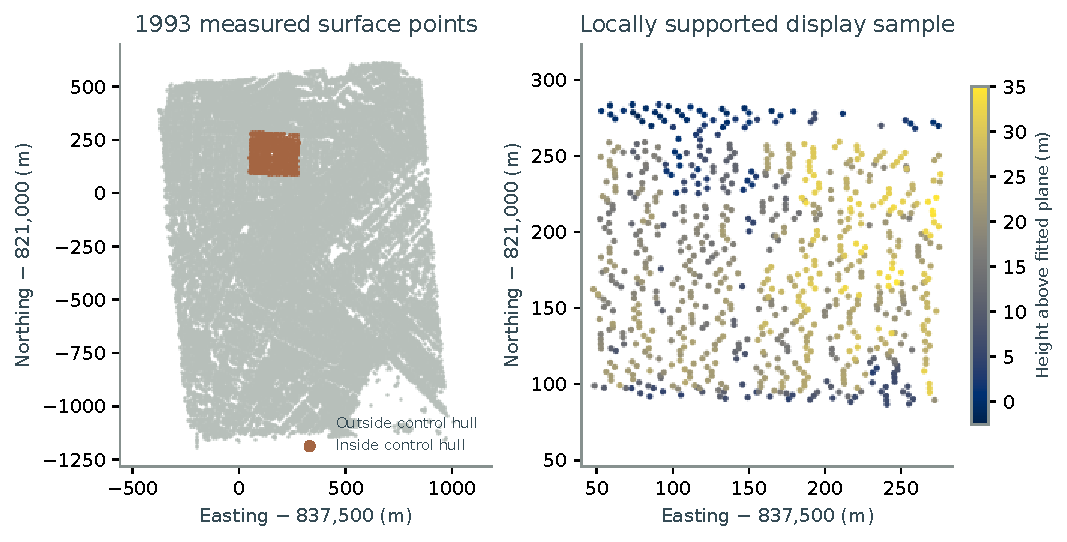
\includegraphics[width=\textwidth]{figures/historical_support.pdf}
\caption{Local support in the historical stereo point cloud. Left: deterministic every-fifth display sample of source points, distinguishing points inside the map-control hull from extrapolated points. Right: relative-plane elevations of the within-hull display sample. Coordinates are diagnostic HK1980 Grid positions with stated offsets; the vertical coordinate is not HKPD. Surfaces are unclassified. No missing region is represented as clear airspace. Source: project reconstruction of Lands Department frames A36142/A36143, 2 November 1993.}
\label{fig:stereo}
\end{figure}

The held-out map controls give a horizontal root-mean-square discrepancy of 5.754 metres for the metric stereo alignment. Only 3,781 dense points lie inside the map-control hull. These facts limit the interpretation of a visually extensive cloud: image coverage is much broader than locally controlled geometry. Points can represent roofs, ground, vegetation or mismatches that survive the filters. They do not constitute a classified, watertight city model.

\subsection{From surface evidence to aircraft clearance}
Clearance concerns the aircraft's swept volume and its tracking uncertainty. It cannot be established by checking a single point against a visually plausible surface. Historical building identities, roof geometry, terrain changes, occlusions, datum offsets and registration errors must be reconciled over the relevant corridor. Unknown geometry must remain unknown rather than becoming an empty obstacle list.

A useful intermediate output is nevertheless possible: an evidence-linked reconstruction in which each object or point records its source date, coordinate meaning and support. Such a resource allows errors to be inspected and corrected. The mathematical landing model can consume it only when the geometric assumptions required by that model are justified.

\status{Dated registered maps and conditional local stereo geometry are available. A complete historical obstacle surface with independently defensible vertical accuracy and whole-aircraft clearance is not established.}

\section{A coupled approach-to-stop model}
\label{sec:model}
\subsection{Why the phases must be considered together}
Turning, descending and slowing compete for time, distance and force. At a given airspeed, tighter turning generally raises lateral force demand. Extending the airborne path can change where the aircraft reaches the runway and how much flare distance is needed. Touchdown speed then enters the stopping law quadratically. An approach model that ends at threshold capture omits part of the constraint interaction.

The current research model uses a coordinated three-dimensional point mass. Its aircraft identity is historically anchored, but its drag, lift, thrust, rate and braking limits are stipulated scenario parameters. It does not include full attitude dynamics, sideslip, landing-gear mechanics or a calibrated wet-runway model. These simplifications make an auditable benchmark possible; they also define the limit of its conclusions.

Let $\mathbf r(t)=(x(t),y(t),h(t))$ be position relative to the usable threshold, with $x$ along the runway, $y$ to the right and $h$ above runway level. For known constant wind $\mathbf w$, define
\begin{equation}
\mathbf v=\dot{\mathbf r}-\mathbf w,\qquad V=\|\mathbf v\|,\qquad
\gamma=\arcsin(v_h/V),\qquad \psi=\operatorname{atan2}(v_y,v_x).
\end{equation}
Inverse dynamics maps a smooth position curve into required lift, bank and thrust. The model then tests those demands against its operating limits, including bank-angle rate and thrust slew. A smooth curve can fail those tests. Appendix~\ref{app:dynamics} gives the equations and distinguishes forward numerical replay from continuous-time certification.

The baseline has zero nominal wind. Constant-wind inverse dynamics cannot be extended to time-varying gusts simply by changing the position equation: air-relative acceleration then also involves wind acceleration. The current mathematical result does not claim that extension.

\subsection{An explicit trajectory family}
The airborne path has approach and flare phases. In each phase, normalized time $s=(t-t_i)/T_i$ lies in $[0,1]$, and
\begin{equation}
\mathbf r_i(t)=\sum_{k=0}^{7}\mathbf c_{ik}s^k.
\label{eq:poly}
\end{equation}
Endpoint-constrained Hermite terms and shape adjustments enforce the selected boundary states. Twelve parameters govern durations, touchdown state and interior shape. Position, velocity and acceleration match at the approach--flare join. The threshold state is an intermediate target, followed by flare, touchdown, a fixed braking delay and constant deceleration.

An explicit polynomial representation is useful because it exposes derivatives and permits interval evaluation. It is not, by itself, a closed-form optimizer. The displayed candidate is one fixed set of coefficients, not a solved function assigning a trajectory to every initial state, wind and dated scene.

\subsection{The objective and its meaning}
Let $g_j\geq0$ denote operating inequalities and let $s_j>0$ be their prescribed normalization scales. The primary criterion is
\begin{equation}
\max_{q,\eta}\ \eta\quad\text{subject to}\quad
\frac{g_j(t;q)}{s_j}\geq\eta\ \text{for all relevant }t,j,
\label{eq:objective}
\end{equation}
with structural equalities and additional hard constraints enforced separately. Here $q$ is the finite parameter vector. A secondary objective minimizes integrated squared normalized bank and rate demands within the specified tolerance of the best primary score.

The score $\eta$ is a normalized model margin. Its value depends on the chosen scales and constraints. It is not an accident probability, a distance clearance or a universal measure of safety. Individual physical margins remain necessary for interpretation. An optimizer that improves on an infeasible numerical seed has constructed a better numerical candidate; it has not outperformed a valid historical flight.

\section{What the synthetic benchmark establishes}
\label{sec:results}
\subsection{A complete feasible candidate within the stated model}
The retained continuous-time certificate evaluates the exact real-decimal candidate through outward-rounded interval arithmetic. It checks a complete cover of both airborne phases, force and rate demands, endpoint conditions and the ground rule. Its 2,502 accepted closed subintervals support a normalized margin of at least 0.0397. The obstacle set in this certificate is empty. Its corridor is a stipulated reference cloud, not a surveyed historical corridor.

\begin{figure}[H]
\centering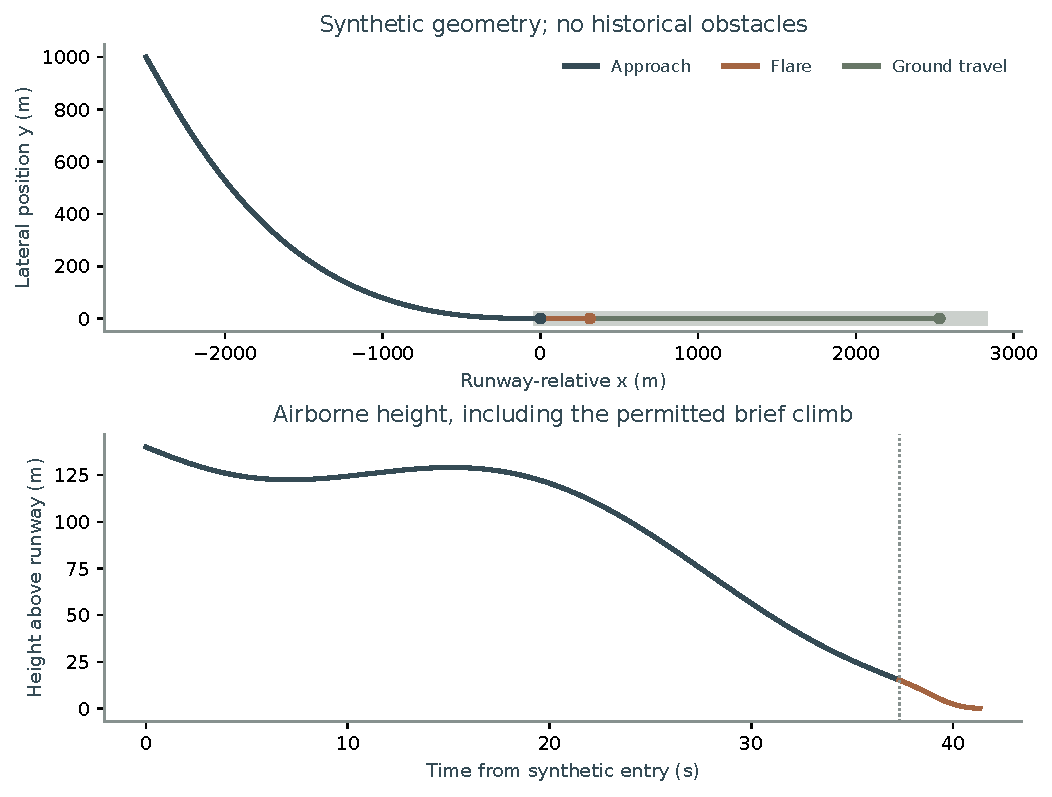
\includegraphics[width=\textwidth]{figures/synthetic_trajectory.pdf}
\caption{The explicit synthetic candidate. Plan view and airborne height are evaluated directly from the frozen coefficient export; the stopping segment uses the fixed braking law. This runway-relative frame is not geographically registered. The brief climb is permitted by the model and is shown rather than described as monotone descent. No historical terrain or buildings are included.}
\label{fig:trajectory}
\end{figure}

\begin{table}[H]
\centering
\caption{Deterministic outcomes of the fixed synthetic candidate. Rounding is for readability; no physical prediction interval is attached.}
\begin{tabular}{@{}lr@{}}
\toprule
Quantity & Scenario value\\
\midrule
Entry to threshold & 37.34 s\\
Flare & 4.00 s\\
Entry to touchdown & 41.34 s\\
Touchdown station beyond usable threshold & 313.49 m\\
Forward touchdown speed & 77.89 m/s\\
Ground travel, including braking delay & 2,217.83 m\\
Threshold-to-stop station & 2,531.32 m\\
Runway remaining & 254.68 m\\
Excess over stipulated 150 m reserve & 104.68 m\\
Entry to complete stop & 96.29 s\\
\bottomrule
\end{tabular}
\label{tab:outcomes}
\end{table}

Independent forward replay reported maximum discrepancies below $1.45\times10^{-7}$ metres in position and $4.04\times10^{-8}$ metres per second in speed. These are numerical consistency measures. They do not estimate physical aircraft accuracy, which is governed by model adequacy and calibration. Likewise, a certificate for the exact source expressions is not automatically a certificate for coefficients rounded in a printed table.

\subsection{Existence and an unresolved performance gap}
Within the specified compact parameter box, a regularity argument bounds vertical speed and excludes inverse-dynamics singularities on the positive-margin feasible domain. Continuity and compactness then establish attainment of the primary maximum. An analogous argument establishes attainment of the secondary minimum on the appropriate restricted set. These are existence results within the selected polynomial family, not formulas for the optimizers.

A separate necessary-condition argument uses the minimum flare duration, the vertical-speed bound, the minimum equivalent airspeed and the stopping constraint. It gives
\begin{equation}
0.0397\leq\eta^*<0.1559772.
\label{eq:bracket}
\end{equation}
The witness and upper bound therefore leave an absolute objective-score gap below 0.1162772. This is not a sufficiently tight result to describe the candidate as near-optimal. Appendix~\ref{app:bounds} records the argument and its domain.

Earlier tighter bounds from defective global-exclusion calculations were withdrawn. They are not used anywhere in this manuscript. Retaining that correction is important: a successful local solve, or a global search that stops with unresolved regions, cannot replace a valid upper bound. The surviving feasible witness and the independent scalar upper bound answer different questions and remain separate.

\subsection{A transparent stopping calculation}
For touchdown station $x_D$, forward speed $u$, delay $d$, deceleration $a>0$ and usable length $L$, the stipulated ground model gives
\begin{equation}
S=x_D+ud+\frac{u^2}{2a},\qquad R=L-S,
\label{eq:stop}
\end{equation}
where $S$ is threshold-to-stop consumption and $R$ is runway remaining. Differentiation yields
\begin{equation}
\frac{\partial R}{\partial x_D}=-1,\quad
\frac{\partial R}{\partial u}=-d-\frac ua,\quad
\frac{\partial R}{\partial d}=-u,\quad
\frac{\partial R}{\partial a}=\frac{u^2}{2a^2}.
\end{equation}
At the fixed candidate, an extra metre of touchdown distance removes one metre of remaining runway. The local sensitivity to a one-metre-per-second increase in touchdown speed is approximately 54.95 metres of lost runway; an extra second of delay costs approximately 77.89 metres if the other inputs are held fixed. These are partial derivatives of an illustrative stopping law, not effects estimated from accident data. The airborne trajectory may not permit the inputs to vary independently.

\begin{figure}[H]
\centering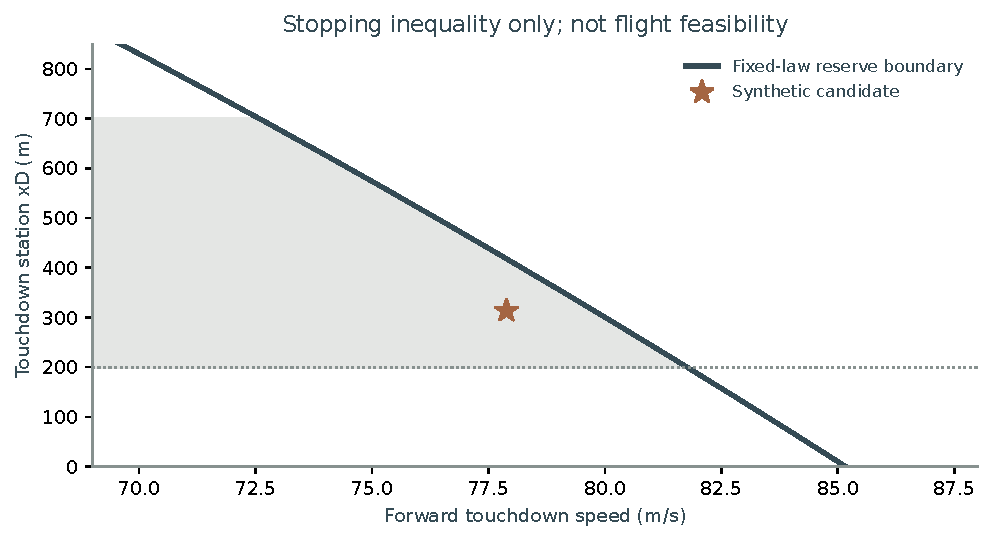
\includegraphics[width=0.93\textwidth]{figures/stopping_boundary.pdf}
\caption{Conditional stopping boundary under the fixed law. The curve shows the latest touchdown station consistent with the stipulated 150 m reserve, as a function of forward touchdown speed. Delay is 2 s, deceleration is $1.4709975$ m/s$^2$, and available length is 2,786 m. The shaded region satisfies this scalar stopping inequality only; it is not an airborne-feasibility region. The star marks the synthetic candidate.}
\label{fig:stop}
\end{figure}

This calculation illustrates why touchdown location and speed belong in the same problem as the approach. It does not demonstrate that speed can be reduced safely at any desired point, that stronger braking is available, or that a historical crew had the information and controls assumed by a counterfactual optimizer.

\section{Historical weather and the validation problem}
\label{sec:weather}
The retained NOAA Integrated Surface Database archive contains 8,549 records for station identifiers 450070--99999 in 1993, including 24 records on 4 November \cite{noaa,isd}. Decoding preserves source flags, missing values and raw fields. A record containing missing wind is not converted to calm conditions, and absence of a gust group is not interpreted as zero gust.

For descriptive comparison, the routine subset is fixed to FM-15 reports with source flag 4, exact UTC-hour timestamps, normal-wind coding, present wind speed with quality code 1 or 5, and exclusion of rows missing both temperature and visibility. It contains 8,360 observed records. This is a selected archive subset, not a random sample of landings or a complete set of independent weather states.

The 03:00 and 04:00 UTC reports on 4 November both give wind from $070^\circ$ true at 10.8 m/s, approximately 21 knots. Their structured gust values are 17.5 and 20.6 m/s, respectively. Agreement of the mean values with the CAD published mean is cross-source consistency; the sources may derive from the same originating observations. Neither hourly value establishes the instantaneous three-dimensional wind acting on the aircraft between reports.

\begin{figure}[H]
\centering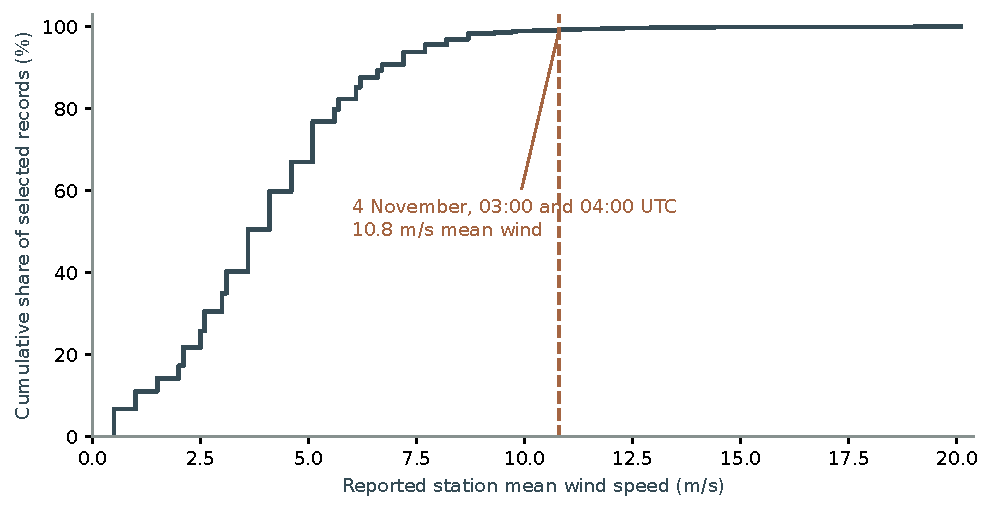
\includegraphics[width=0.94\textwidth]{figures/weather_context.pdf}
\caption{Observed routine station-wind context in 1993. The empirical cumulative distribution uses the declared 8,360-record subset. At 10.8 m/s, 8,285 records are strictly lower, 17 tie and 58 are higher. Serial dependence, missing hours and selection rules preclude interpreting the display as an accident probability, return period or distribution of aircraft-local wind. Source: decoded NOAA ISD 450070--99999 archive.}
\label{fig:weather}
\end{figure}

The case therefore challenges the model in a non-benign observed weather context. But it does not calibrate a gust process. Station siting, sensor height, the relation between surface measurements and aircraft-local wind, and clock offsets remain material. A high rank in the annual routine subset cannot identify which wind realization acted along the flight path.

The matched-case reconstruction will preserve separate wind-system and flight-recorder clocks until an alignment is supported. Published narrative events can cross-check digitized curves, but they are not necessarily independent measurements. A comparison to the zero-wind synthetic witness must expose the mismatched conditions rather than interpreting the distance between the curves as pilot inefficiency.

\status{The weather decoder, retained tables and quality checks are complete for this source snapshot. The combined flight/weather reconstruction, model discrepancy analysis and routine-flight validation are not results of this first draft.}

\section{Uncertainty, counterfactuals and the meaning of a better approach}
\label{sec:uncertainty}
\subsection{Different errors require different evidence}
Measurement error concerns observed inputs, such as positions or a plotted speed trace. Model discrepancy concerns the difference between the chosen aircraft equations and real dynamics. Approximation error concerns a compact rule's difference from its reference computation. Tracking error concerns an aircraft's departure from the planned reference. An optimality gap concerns the distance between achieved and best admissible objective values. These cannot be compressed into one numerical band without a joint model and supporting evidence.

For example, a terrain product's stated accuracy at a confidence level does not supply a worst-case obstacle bound. An interval-arithmetic proof controls numerical enclosure under its assumptions, not the correctness of the assumptions. A held-out horizontal map-control error does not independently calibrate vertical roof error. Each number must retain the question it answers.

\subsection{What deterministic envelopes already provide}
Suppose evidence supplies a joint enclosing box for $x_D,u,d,a,L$, with positive lower deceleration and nonnegative speed and delay. Monotonicity of equation~\eqref{eq:stop} gives
\begin{align}
S_-&=x_-+u_-d_-+\frac{u_-^2}{2a_+},&
S_+&=x_++u_+d_++\frac{u_+^2}{2a_-},\\
R&\in[L_- -S_+,\ L_+-S_-].
\end{align}
These are exact extrema over the Cartesian box for the stated scalar law. Dependence or flight constraints can make the range conservative. Statistical independence is not assumed. No physical box has been calibrated for this manuscript, so the formulas do not justify attaching a numerical physical band to Table~\ref{tab:outcomes}.

A prediction interval for an individual landing requires a justified conditional distribution for the outcome and validation in the intended domain. It differs from a confidence interval for a mean or an estimated coefficient. Marginal intervals for touchdown and stopping do not automatically provide joint coverage, and endpoint coverage does not establish clearance along an entire path.

\subsection{The information available to a candidate matters}
An offline optimizer may be given an entire future wind history. A pilot or causal controller cannot use unobserved future disturbances. The distinction can be written as
\begin{equation}
\exists\pi\ \forall w\in\mathcal W:\ \text{constraints hold}
\qquad\text{versus}\qquad
\forall w\in\mathcal W\ \exists\pi_w:\ \text{constraints hold}.
\end{equation}
The second statement permits a different solution after each complete wind realization is known. It is weaker than a single admissible policy that works across the disturbance set. A fair historical comparison must specify the information set, response limitations and navigation aids as well as aircraft dynamics.

The primary counterfactual should keep aircraft, mass, entry state, runway, dated obstacles, braking, operating limits and available information fixed. A modern-guidance comparison can be useful, but is a separately labelled question. A candidate can only disprove the optimality of a particular baseline if both are feasible for the same problem and its strict advantage exceeds relevant uncertainty.

\section{Relation to existing research and contribution to Hong Kong}
\label{sec:contribution}
\subsection{Where the research sits}
Aircraft trajectory optimization, bounded-curvature planning and robust tracking are established subjects. Wu and Chen characterize minimum-time paths for a Dubins airplane in steady wind; some candidate families reduce to quadratic equations and others require transcendental root finding \cite{wu}. That reduced setting is a valuable benchmark, not a complete descending landing with flare and stopping.

Kim and coauthors study six-degree-of-freedom landing trajectories with runway alignment, obstacles and constant wind using sequential convex programming \cite{kim}. That provides a substantially richer dynamics comparator. FaSTrack separates a simplified planner from tracking dynamics and a tracking-error bound \cite{fastrack}. Its demonstrations do not certify a Kai Tak airliner, but the distinction between planned geometry and trackable motion is directly relevant here.

The present paper does not claim novelty merely from applying optimization to Kai Tak. Its prospective addition is the combination of a documented historical benchmark, explicit approximate trajectory rules, transparent performance bounds and uncertainty-aware confrontation with records. Each element must be evaluated against its own literature. The current screening is bounded rather than exhaustive, and the comparative algorithms have not been reproduced in this version.

\subsection{A useful historical research resource}
The immediate public value lies in making a difficult historical engineering problem inspectable. A dated source catalogue and reconstruction can support aviation-history teaching. An explicit model can show students why reaching the runway is not the same as completing a landing. A reproducible analysis can help future researchers distinguish a missing input from a mathematical impossibility.

The intended public package would include the white paper, authored code, provenance records and explanatory visualizations, subject to source rights. It would distinguish original materials from derived artifacts and preserve gaps rather than inventing completeness. This version has not been publicly released, and no external adoption or societal impact is claimed. Potential uses are not evidence that those uses have already occurred.

The work's relevance to Hong Kong follows from its object: the geometry, records and engineering history of a particular place. A generalizable mathematical method would be an additional contribution, not a prerequisite for a careful historical dataset to be useful. Contemporary aviation applications would require separate validation.

\section{Limitations and the next version}
\label{sec:next}
The first draft has a mathematical candidate and historical evidence, but not yet a historical candidate validated against that evidence. Its central remaining task is integration under defensible assumptions. It must not close that gap by relabelling a synthetic path, replacing unknown historical obstacles with empty space, or attaching arbitrary probability distributions to uncertain inputs.

\begin{table}[H]
\caption{Evidence needed before the corresponding stronger claim can enter the paper. These are unfinished research requirements, not exclusions from the intended study.}
\small
\begin{tabularx}{\textwidth}{@{}p{0.32\textwidth}X@{}}
\toprule
Proposed claim & Required evidence\\
\midrule
Historical model consistency & Source-linked flight traces; defensible clock, speed and height conventions; explicit model comparison with uncertainty.\\
Terrain-aware feasibility & Registered runway and historical obstacle geometry; datum reconciliation; aircraft-volume and tracking allowance; full-path checks.\\
Useful condition-dependent rule & A declared input domain, validated reference solutions, fitted explicit coefficients and out-of-domain refusal.\\
Near-optimality & A valid, useful objective-gap bound for the same feasible set and objective.\\
Calibrated landing predictions & Supported joint input/discrepancy assumptions and relevant out-of-sample coverage evidence.\\
Historical improvement & A valid baseline and candidate with equivalent conditions and information; an advantage that survives uncertainty.\\
\bottomrule
\end{tabularx}
\end{table}

The immediate empirical priority is the matched CAL605 reconstruction. It can expose inconsistencies in the current model and establish which aspects of the recorded motion are actually identified. It cannot establish typical operational performance from one accident. Broader validation remains dependent on routine approaches, go-arounds and their configuration and weather metadata.

The mathematical priority is a useful certified gap or a clearly scoped approximation result after historical constraints are introduced. Exact symbolic global optimality is not required for the intended study. An explicit approximation with honest error and performance bounds can be more informative than an opaque numerical optimum, provided its domain and limitations are established.

\section{Conclusion}
Kai Tak can be studied as a coupled geometric and dynamical problem without assuming either that its approach was uniquely optimal or that a better one must exist. This first version assembles a dated evidence base, presents conditional historical 3D measurements, constructs an explicit synthetic approach-to-stop candidate and separates its feasibility certificate from the unresolved optimum.

The candidate establishes that the stipulated reduced problem admits a complete landing trajectory. The reconstruction establishes that historical geometry can be recovered locally from actual imagery. The weather diagnostic establishes that the selected accident case occupies an unusually windy part of the declared routine archive subset. None of these results alone resolves the historical landing problem.

The next version should connect them through a common, uncertainty-aware comparison. The contribution will be strongest where a clear statement survives that connection: a physical constraint identified, a historical feature recovered, a model assumption rejected, or an alternative trajectory shown to improve a defined objective under the same conditions. That is the standard by which this project should be judged.

\clearpage
\appendix
\section{Dynamics, parameter domain and explicit construction}
\label{app:dynamics}
\subsection{Inverse and forward equations}
With the definitions in Section~\ref{sec:model}, set
\begin{align}
\mathbf e_V&=(\cos\gamma\cos\psi,\cos\gamma\sin\psi,\sin\gamma),\\
\mathbf e_\gamma&=(-\sin\gamma\cos\psi,-\sin\gamma\sin\psi,\cos\gamma),\\
\mathbf e_\psi&=(-\sin\psi,\cos\psi,0),\qquad
\mathbf f=\ddot{\mathbf r}+(0,0,g).
\end{align}
Writing $\ell_\gamma=\mathbf f\cdot\mathbf e_\gamma$ and $\ell_\psi=\mathbf f\cdot\mathbf e_\psi$, required lift $\mathcal L$, bank $\phi$, drag $D$ and thrust $\mathcal T$ are
\begin{align}
\mathcal L&=m\sqrt{\ell_\gamma^2+\ell_\psi^2},&
\phi&=\operatorname{atan2}(\ell_\psi,\ell_\gamma),\\
C_L&=\frac{2\mathcal L}{\rho V^2 S_w},&
D&=\tfrac12\rho V^2 S_w(C_{D0}+k_D C_L^2),\\
\mathcal T&=m\mathbf f\cdot\mathbf e_V+D,&
\rho(h)&=\rho_0 e^{-h/H_\rho}.
\end{align}
Here $S_w$ is wing area, not stopping station. At nonzero speed, nonzero horizontal airspeed and positive lift, these expressions and their time derivatives define the continuous model's control demands. Bank-angle rate is not automatically body-axis roll rate.

The corresponding forward equations are
\begin{align}
\dot{\mathbf r}&=V\mathbf e_V+\mathbf w,&
\dot V&=(\mathcal T-D)/m-g\sin\gamma,\\
\dot\gamma&=\frac{\mathcal L\cos\phi/m-g\cos\gamma}{V},&
\dot\psi&=\frac{\mathcal L\sin\phi}{mV\cos\gamma}.
\end{align}
Replay integrates these equations using derived commands. For stronger consistency checking, lift can be recomputed from the replayed state and the specified $C_L$ command. A sampled integration can detect disagreement, but does not establish an inequality at every time. The interval certificate addresses that separate numerical question within the same reduced dynamics.

\subsection{Scenario parameters}
\begin{table}[H]
\caption{Stipulated model quantities. These are research assumptions, not manufacturer-approved limits.}
\small
\begin{tabularx}{\textwidth}{@{}XX@{}}
\toprule
Quantity & Value\\
\midrule
Bank / bank-angle rate limits & $25^\circ$ / $5^\circ$ per second\\
Equivalent airspeed band & 135--175 kt\\
Lift coefficient / load-factor bands & 0--2.8 / 0.5--1.4\\
Thrust / thrust-slew limits & 700 kN / 100 kN per second\\
Maximum descent angle & $6^\circ$\\
Maximum approach sink / touchdown sink & 8 / 1.5 m/s; target touchdown sink 0.7 m/s\\
Density reference / scale height & 1.225 kg/m$^3$ / 8,500 m\\
Wing area / drag coefficients & 541.2 m$^2$ / $C_{D0}=0.08$, $k_D=0.045$\\
Synthetic corridor half-width & 400 m around the fixed reference point cloud\\
Threshold height / flight-path angle & 15.24 m / $-3.1^\circ$\\
Ground delay / deceleration / reserve & 2 s / 1.4709975 m/s$^2$ / 150 m\\
\bottomrule
\end{tabularx}
\end{table}

The nominal entry position is $(-2500,1000,140)$ m. Entry and threshold EAS are fixed at 153 kt, with density conversion to true airspeed. The initial ground-track angle is $-47^\circ$ in the synthetic runway frame. Aircraft mass is the exact unit conversion of the source-estimated weight, $238461.67357166$ kg; this numerical exactness does not improve the historical estimate.

The finite parameter box has approach duration $T_A\in[30,55]$ s, flare duration $T_F\in[4,12]$ s, touchdown station $x_D\in[200,700]$ m and forward speed $u\in[69,88]$ m/s. Each of the four horizontal approach-shape amplitudes lies in $[-400,400]$ m; the two vertical amplitudes lie in $[-50,50]$ m. Flare-shape amplitudes lie in $[-50,50]$ m horizontally and $[-10,10]$ m vertically. These parameter restrictions define the family in the attainment and upper-bound statements.

\subsection{Endpoint-preserving polynomials}
For endpoints $p_0,p_1$, velocities $v_0,v_1$, accelerations $a_0,a_1$ and duration $T$, define vector coefficients
\begin{align}
c_0&=p_0,&c_1&=Tv_0,&c_2&=T^2a_0/2,\\
A&=p_1-c_0-c_1-c_2,&B&=Tv_1-c_1-2c_2,&C&=T^2a_1-2c_2,\\
c_3&=10A-4B+C/2,&c_4&=-15A+7B-C,&c_5&=6A-3B+C/2.
\end{align}
The polynomial $P(s)=\sum_{k=0}^5c_ks^k$ satisfies all six endpoint conditions by direct substitution and differentiation. The shape functions
\begin{equation}
B_0(s)=64s^3(1-s)^3,\qquad B_1(s)=(2s-1)B_0(s)
\end{equation}
and their first two derivatives vanish at both endpoints. Adding coordinate-specific multiples of these functions adjusts the interior without changing endpoint position, velocity or acceleration. Their explicit derivatives permit evaluation of inverse forces and rates without spline differentiation. Both one-sided control-rate limits at the phase join must still be checked.

The full-precision floating coefficient export is included in the source package as \path{reference_formula.json}, under \path{evidence/approximation/}. It is an evaluation representation. The certificate instead reconstructs its source expressions from the exact-decimal candidate. The draft figures evaluate the former; the scientific margin claim refers to the latter.

\section{Restricted attainment and the surviving bound}
\label{app:bounds}
\subsection{Why a best member exists}
The retained project proof first establishes $|v_h|<14$ m/s for both vertical-velocity polynomials across the full parameter box. In this appendix $v_h$ denotes vertical velocity; it is distinct from horizontal speed. On the nonnegative-height feasible domain, the lower EAS bound implies total airspeed at least $135(1852/3600)$ m/s. Combined with the vertical-speed bound, this keeps horizontal speed above 68 m/s. The positive load lower bound keeps lift away from zero, and the bank constraints retain the positive-up lift branch.

\begin{proposition}[Attainment in the nominal finite family]
Under the fixed zero-wind scenario, parameter box, continuous constraints, density and force model, corridor cloud and ground rule, the primary maximum is attained. The stipulated secondary continuous-effort minimum is also attained on the retained-primary set.
\end{proposition}
\begin{proof}
The certified candidate makes the set with $\eta\geq0.0397$ nonempty. Restrict $q$ to its compact box and $\eta$ to a closed bounded interval containing the valid lower and upper bounds. Along any convergent feasible sequence, the polynomial states and derivatives through jerk converge uniformly, since durations remain bounded away from zero. The regularity bounds above prevent speed, lift and angular-coordinate singularities at the limit. Inverse forces, exact rates and the relevant margins therefore pass continuously to the limit. Distance to the fixed finite reference cloud is continuous. Every time-indexed inequality and terminal constraint is preserved, so the feasible set is closed and bounded. The continuous coordinate function $\eta$ attains a maximum on it. The continuous integrated effort attains a minimum on its nonempty closed subset retaining the primary optimum within $10^{-4}$.
\end{proof}
This argument does not evaluate the maximizing parameters. It does not extend automatically to unrestricted control functions, other winds or historical obstacles. The underlying vertical-speed enclosure and candidate certificate are computer-assisted results retained with the evidence snapshot, not a newly performed independent proof audit in this typesetting task.

\subsection{A necessary upper bound from flare and stopping}
Let $\kappa=1852/3600$ and define
\begin{equation}
u_{\min}(\eta)=\sqrt{[\kappa(135+40\eta)]^2-0.7^2}.
\end{equation}
At touchdown the density is $\rho_0$, lateral speed is zero and the vertical speed is $-0.7$ m/s. The normalized EAS margin therefore requires $u\geq u_{\min}(\eta)$. During flare, zero lateral motion, nonnegative height and the global vertical-speed bound require
\begin{equation}
v_x\geq\sqrt{[\kappa(135+40\eta)]^2-14^2}.
\end{equation}
Because $T_F\geq4$ s and flare begins at $x=0$, the touchdown station is at least four times this lower speed. The normalized stop margin requires $S\leq2636(1-\eta)$, where $2636=2786-150$. Combining these necessary conditions gives
\begin{multline}
4\sqrt{[\kappa(135+40\eta)]^2-14^2}
+2u_{\min}(\eta)+\frac{u_{\min}(\eta)^2}{2(1.4709975)}\\
\leq2636(1-\eta).
\end{multline}
The difference between the left and right sides is strictly increasing for $\eta\geq0$. Outward-rounded source evaluation brackets its root between 0.1559771 and 0.1559772. Thus every feasible member of this family has $\eta<0.1559772$.

With the candidate lower certificate, this yields equation~\eqref{eq:bracket}. No equality-achieving candidate or tight global secondary certificate has been established. The previously withdrawn 0.03972 bound is excluded. A search that leaves unexcluded parameter boxes cannot sharpen the bound by treating those boxes as impossible.

\section{Ground motion and conditional outcome ranges}
\label{app:ground}
Let $t_D=T_A+T_F$ and $q_g=t-t_D$. The ground phase is
\begin{equation}
x(t)=\begin{cases}
x_D+uq_g,&0\leq q_g\leq d,\\
x_D+ud+u(q_g-d)-\tfrac12 a(q_g-d)^2,&d\leq q_g\leq d+u/a.
\end{cases}
\end{equation}
The solution ends at rest. Vertical velocity is reset at touchdown by the stipulated contact rule, which does not resolve landing-gear impact dynamics. Total entry-to-stop time is
\begin{equation}
t_{\mathrm{stop}}=T_A+T_F+d+u/a.
\end{equation}
If $T_A\in[A_-,A_+]$ and $T_F\in[F_-,F_+]$, along with the scalar box in Section~\ref{sec:uncertainty}, then
\begin{equation}
t_{\mathrm{stop}}\in
\left[A_-+F_-+d_-+\frac{u_-}{a_+},\quad
A_++F_++d_++\frac{u_+}{a_-}\right].
\end{equation}
The extrema follow from monotonicity for $a_->0$, $u_-\geq0$ and $d_-\geq0$. Exact rational endpoint arithmetic can enclose these calculations without assuming a probability distribution. Whether the extreme combinations correspond to feasible airborne trajectories is a separate issue. The present numerical test boxes verify software and algebra, not real-world uncertainty coverage.

\section{Provenance, reproducibility and author review}
\label{app:provenance}
\subsection{Evidence frozen for this version}
The companion source package contains a timestamped SHA-256 manifest and snapshots of the project reports used in the manuscript. It also contains reduced numerical inputs for the five figures. Original third-party report PDFs, survey imagery and full aerial photographs are not bundled. Their primary-source identities and retrieval routes remain documented.

\small
\begin{longtable}{@{}>{\raggedright\arraybackslash}p{0.31\textwidth}>{\raggedright\arraybackslash}p{0.62\textwidth}@{}}
\toprule
Claim group & Source record in the project\\
\midrule\endhead
Historical geometry and recorder limitations & \path{evidence/EVIDENCE_REPORT.md}; CAD Report 1/95, sections 1.6, 1.8--1.11, 2.6.5 and Appendices 1, 11--12.\\
Map acquisition and chronology & \path{reconstruction/chronology/REPORT.md}; \path{reconstruction/block_matching/registration_report.md}.\\
Conditional stereo reconstruction & \path{reconstruction/block_matching/aerial_registration/README.md}, sparse/dense reports and \path{stereo_verification.json}.\\
Aircraft assumptions and objective & \path{MODEL_IMPLEMENTATION_SPEC.md}; \path{MODEL_EQUATIONS.md}; \path{model/config.json}.\\
Feasible candidate and family bounds & \path{analytical/coupled/RESULTS.md}; \path{continuous_certificate_refined.json}.\\
Explicit formula and scenario outcomes & \path{approximation/reference_formula.json}; \path{reference_outcomes.json}; \path{CLOSED_FORM_AND_BOUNDS.md}.\\
Selected flight/weather findings & \path{evidence/cal605_reconstruction/REPORT.md}, \path{analysis.json}, \path{verification.json}; primary CAD source landmarks cross-checked.\\
Annual weather selection & \path{evidence/cal605_reconstruction/noaa/README.md}, \path{verification.json} and \path{acceptance_verification.json}.\\
Scope of related-work screening & \path{literature/LITERATURE_AND_COMPARISON.md}; \path{APPROXIMATE_LANDING_NOVELTY_2026-10-13.md}.\\
\bottomrule
\end{longtable}
\normalsize

The draft builder checks the frozen artifact hashes, recomputes the scalar stopping outcomes, evaluates airborne endpoints and reproduces the weather subset counts before drawing figures. PDF checks cover citations, text extraction, page geometry and fonts. These document checks do not constitute a new independent scientific review of the source certificates or photogrammetric reconstruction.

\subsection{Research and drafting contributions}
Aryan Ayyar initiated the research question and set the project's scientific direction. The computational workflows, reconstruction, verification records and manuscript have been developed with AI-assisted research, coding and drafting. This first version is prepared for his substantive review; it should not imply that all derivations have already been independently checked by a human specialist. Any later contribution or acknowledgement statement should reflect the work and reviews actually completed.

The document is an independent working white paper. No university, aviation authority or archive is represented as endorsing its results. Public release, third-party-material reuse and any external review are separate steps from producing this private draft. Source attribution does not imply unrestricted redistribution rights.

\subsection{Version record}
Version 1 freezes the restricted mathematical result, corrected conditional historical reconstruction and settled exploratory CAL605 flight/weather benchmark. The final drafting check incorporated the reconstruction's 49-point correction and the newly completed benchmark after verifying their handoff hashes. Later versions should identify changed evidence, revised claims and any superseded result explicitly. Historical feasibility, calibrated uncertainty and improvement requirements remain in scope.

\clearpage
\addcontentsline{toc}{section}{References}
\begin{thebibliography}{9}
\bibitem{cad} Hong Kong Civil Aviation Department (1995).
\emph{Aircraft Accident Report 1/95: Boeing 747-409B, registration B-165, Hong Kong International Airport, 4 November 1993}. August 1995. Primary report; retained 226-page scan from the University of Hong Kong Libraries collection. \href{https://web.archive.org/web/20180517095657id_/http://ebook.lib.hku.hk/HKG/B35838838.pdf}{Archived report}.

\bibitem{dtm} Lands Department, Government of the Hong Kong SAR (2019).
\emph{Key features of DTM: 5m-grid Digital Terrain Model}. Product specification; revision March 2019, photography January--February 2014 and January 2015. \url{https://www.landsd.gov.hk/en/spatial-data/open-data/kf_dtm.html}.

\bibitem{buildings} Lands Department, Government of the Hong Kong SAR (2026).
\emph{Building spatial data}, release metadata dated 21 September 2026. CSDI Portal. Source metadata and snapshot retained in the project. \href{https://portal.csdi.gov.hk/csdi-webpage/metadata/landsd_rcd_1637211194312_35158/html}{Dataset metadata}.

\bibitem{noaa} NOAA National Centers for Environmental Information.
\emph{Integrated Surface Database, station-year file 450070--99999, 1993}. Retained archive acquired 13 October 2026. \url{https://www.ncei.noaa.gov/pub/data/noaa/1993/450070-99999-1993.gz}.

\bibitem{isd} NOAA National Centers for Environmental Information.
\emph{Integrated Surface Data format documentation}. Retained specification used for fixed-width fields, additional groups, missing values and quality flags. \url{https://www.ncei.noaa.gov/pub/data/noaa/isd-format-document.pdf}.

\bibitem{wu} Wu, F., and Chen, Z. (2024).
\emph{Closed-Form Solutions for Minimum-Time Paths of Dubins Airplane in Steady Wind}. arXiv:2412.04797v1. \url{https://arxiv.org/abs/2412.04797v1}.

\bibitem{kim} Kim, T., Kamath, A. G., Rahimi, N., Corleis, J., Açıkmeşe, B., and Mesbahi, M. (2024).
\emph{Six-Degree-of-Freedom Aircraft Landing Trajectory Planning with Runway Alignment}. arXiv:2405.16680v1. The discussion refers to the screened version; a revised version was posted in 2025. \url{https://arxiv.org/abs/2405.16680v1}.

\bibitem{fastrack} Chen, M., Herbert, S. L., Hu, H., Pu, Y., Fisac, J. F., Bansal, S., Han, S., and Tomlin, C. J. (2021).
\emph{FaSTrack: a Modular Framework for Real-Time Motion Planning and Guaranteed Safe Tracking}. arXiv:2102.07039v2; associated journal DOI: \href{https://doi.org/10.1109/TAC.2021.3059838}{10.1109/TAC.2021.3059838}. \url{https://arxiv.org/abs/2102.07039v2}.
\end{thebibliography}

\end{document}
